% --------------------------------------------------------------
% This is all preamble stuff that you don't have to worry about.
% Head down to where it says "Start here"
% --------------------------------------------------------------
 
\documentclass[12pt]{article}
 
\usepackage[margin=1in]{geometry} 
\usepackage{amsmath,amsthm,amssymb}
\usepackage{mathtools}
\usepackage{graphicx}
\usepackage{tikz}
\usepackage{subfig}
\usepackage{tcolorbox}
 
\newcommand{\N}{\mathbb{N}}
\newcommand{\Z}{\mathbb{Z}}
 
\newenvironment{theorem}[2][Theorem]{\begin{trivlist}
\item[\hskip \labelsep {\bfseries #1}\hskip \labelsep {\bfseries #2.}]}{\end{trivlist}}
\newenvironment{lemma}[2][Lemma]{\begin{trivlist}
\item[\hskip \labelsep {\bfseries #1}\hskip \labelsep {\bfseries #2.}]}{\end{trivlist}}
\newenvironment{exercise}[2][Exercise]{\begin{trivlist}
\item[\hskip \labelsep {\bfseries #1}\hskip \labelsep {\bfseries #2.}]}{\end{trivlist}}
\newenvironment{reflection}[2][Reflection]{\begin{trivlist}
\item[\hskip \labelsep {\bfseries #1}\hskip \labelsep {\bfseries #2.}]}{\end{trivlist}}
\newenvironment{proposition}[2][Proposition]{\begin{trivlist}
\item[\hskip \labelsep {\bfseries #1}\hskip \labelsep {\bfseries #2.}]}{\end{trivlist}}
\newenvironment{corollary}[2][Corollary]{\begin{trivlist}
\item[\hskip \labelsep {\bfseries #1}\hskip \labelsep {\bfseries #2.}]}{\end{trivlist}}
\newenvironment{question}[2][Question]{\kern10pt \begin{trivlist}
\begin{tcolorbox}
\item[\hskip \labelsep {\bfseries #1}\hskip \labelsep {\bfseries #2.}]}
{\end{tcolorbox} \end{trivlist}}
 
\newcommand\mytodo[1]{\textcolor{red}{#1}}

\newcommand*{\answer}{%
  \par
  \kern1pt
  \begingroup
    \centering
    \raisebox{.2\baselineskip}{%
      \textcolor{gray}{
	    \rule{.6667\linewidth}{.1pt}%
      }
    }%
    \par
  \kern8pt
  \endgroup
}

\begin{document}
 
\graphicspath{ {img/} }
% --------------------------------------------------------------
%                         Start here
% --------------------------------------------------------------
 
\renewcommand{\qedsymbol}{\filledbox}
 
\title{Machine Learning, Advanced Course (DD2434)\\
		Assignment 2}
\author{Martin Hwasser, hwasser@kth.se}
 
\maketitle

\begin{question}{1}

In which pairs is one value larger than the other?
\end{question}
$$p(t^1 \vert d^1) < p(t^1)$$
$$p(d^1 \vert t^0) > p(d^1)$$
$$p(h^1 \vert e^1, f^1) > p(h^1 \vert e^1)$$
$$p(c^1 \vert h^0) < p(c^1)$$

\begin{question}{2}
Which pairs are equal?
\end{question}
$$p(c^1 \vert f^0) = p(c^1)$$
$$p(d^1 \vert h^1, e^0) = p(d^1 \vert h^1)$$
$$p(c^1 \vert h^0, f^0) = p(c^1 \vert h^0)$$

\begin{question}{3}
Which pairs are incomparable (i.e., the two values can not be compared based on the information available in the DAG.)
\end{question}
\begin{center}
$p(d^1 \vert e^1, f^0, w^1)$ and $p(d^1 \vert e^1, f^0)$
\\
$p(t^1 \vert w^1, f^0)$ and $p(t^1 \vert w^0)$
\end{center}

\begin{question}{6}
Provide data generated using at least three different sets of categorical dice distributions – what does it look like for all unbiased dice, i.e., uniform distributions, for example, or if some are biased in the same way, or if some are unbiased and there are two different groups of biased dice.
\end{question}

Figure \ref{casino_fair} shows the distribution of outcomes when the dices of both the casino and the players have a uniform distribution.

Figure \ref{casino_c_unfair} shows the distribution of outcomes when players have fair dices, but the primed tables have a distribution like $p(1) = \frac{5}{10}$ and $p(1>) = \frac{1}{5}$.

Figure \ref{casino_p_unfair} shows the distribution of outcomes when the casino have biased dices like in \ref{casino_c_unfair}, but the players also have a biased distribution $p(<6) = \frac{1}{7}$ and $p(6) = \frac{2}{7}$.

\begin{figure}
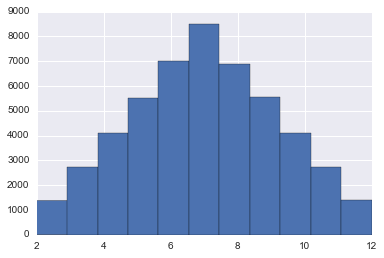
\includegraphics[]{casino_fair}
\centering
\caption{Both casino and player have fair dices.}
\label{casino_fair}
\end{figure}

\begin{figure}
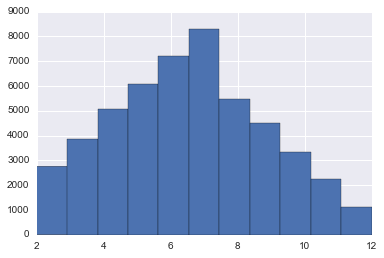
\includegraphics[]{casino_c_unfair}
\centering
\caption{The casino has unfair dices on certain tables.}
\label{casino_c_unfair}
\end{figure}

\begin{figure}
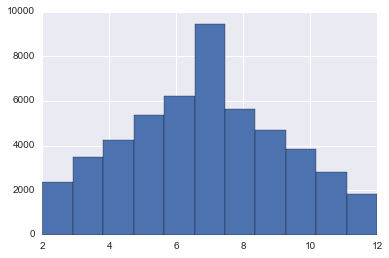
\includegraphics[]{casino_p_unfair}
\centering
\caption{Both the casino and the players have unfair dices.}
\label{casino_p_unfair}
\end{figure}


\begin{question}{8}
Describe the exact posterior.
\end{question}
%$$p(\mu, \lambda) = \mathcal{N}(\mu \vert \mu_0 (\beta\lambda)^{-1} Gam(\lambda \vert a,b)$$
%where $\mu_0 = c/\beta, a = 1 + \beta/2, b = d-c^2/2\beta.$
\begin{align}
\begin{split}
p(\mu, \lambda \vert D) &= \mathcal{NG}(\mu, \lambda \vert \mu_n, \kappa_n, \alpha_n, \beta_n)
\\
\mu_n &= \frac{\kappa_0 \mu_0 + n \bar{x}}{k_0 + n}
\\
\kappa_n &= \kappa_0 + n
\\
\alpha_n &= \alpha_0 + n/2
\\
\beta_n &= \beta_0 + \frac{1}{2} \sum_{i=1}^{n} (x_i - \bar{x})^2 + \frac{\kappa_0 n (\bar{x} - \mu_0)^2}{2(\kappa_0 + n)}
\end{split}
\end{align}

\begin{question}{9}
Compare the variational distribution with the exact posterior. Run the inference
for a couple of interesting cases and describe the difference.
\end{question}

In figure \ref{q9} we see both the true posterior, and the approximated posterior.

\begin{figure}
\includegraphics[]{q9}
\centering
\caption{Variational inference.}
\label{q9}
\end{figure}

\begin{question}{10}
Describe an algorithm that, given (1) the parameters $\Theta$ of the full casino model of Task 2.2 (so, Θ is all the categorical distributions corresponding to all the dice), (2) a sequence of tables $r_1,...,r_K$ (that is, $r_i$ is $t_i$ or $t'_i$) , and (3) an observation of dice sums $s_1,..., s_K$, outputs
$p(r_1,..., r_K \vert s_1,..., s_K, \Theta)$.
\end{question}

\begin{equation}
\begin{split}
p(r_1,..., r_K \vert s_1,..., s_K, \Theta) &= \big\{ \text{Product rule} \big\} 
\\
&= \frac{p(r_1,...,r_K, s_1,...,s_K, \Theta)}{p(s_1,...,s_K, \Theta)}
\\
&= \big\{\text{Bayes' theorem}\big\}
\\
&= \frac{p(s_1,...,s_K \vert r_1,...,r_K, \Theta) p(r_1,...,r_K, \Theta)}{p(s_1,...,s_K, \Theta)}
\end{split}
\end{equation}

The sum of the two dice rolls depend both on the player's dice distribution and the table's dice distribution:

\mytodo{omit $\Theta$ and say it's fixed?}
\begin{equation}
\begin{split}
p(s_1, ..., s_K \vert r_1, ..., r_K, \Theta) &= p(s_1,...,s_{K-1} \vert s_K, r_1, ..., r_K)
\\
&=p(s_1, ..., s_{K-1} \vert r_1, ..., r_K) p(s_k \vert r_K)
\\
&=p(s_1,...,s_{K-2} \vert s_{K-1}, r_1, ..., r_K) p(s_{K-1} \vert r_1,...,r_K)p(s_K \vert r_K)
\\
&=p(s_1, ..., s_{K-2} \vert r_1, ..., r_K) p(s_{K-1} \vert r_{K-1}) p(s_{K} \vert r_K)
\\
&=\prod_{k=1}^{K} p(s_k \vert r_k, \Theta)
\\
&= \prod_{k=1}^{K} \sum_{x=1,y=1}^{6} \boldsymbol{1}_{s_k}(x + y) (X_k = x \vert \Theta) (Y_k = y \vert \Theta)
\\
&= \prod_{k=1}^{K} \sum_{x=1,y=1}^{6} \boldsymbol{1}_{s_k}(x + y) MN(x \vert \beta) MN(y \vert \gamma)
\end{split}
\end{equation}

where $MN$ is the multinoulli, or categorical distribution.

Knowing that the table's dice distribution only depends on the previous table's dice distribution, and as such has the first order Markov property, we can express this by:

\mytodo{omit $\Theta$ and say it's fixed?}
\begin{equation}
\begin{split}
p(r_1,...,r_K \vert \Theta) &= p(r_2, r_3, ..., r_K \vert r_1)p(r_1)
\\
&= p(r_3,...,r_K \vert r_2)p(r_2 \vert r_1) p(r_1)
\\
&=p(r_1, \Theta) \prod_{k=2}^{K} p(r_k \vert r_{k-1}, \Theta)
\end{split}
\end{equation}

\mytodo{look this over}

We can take the first initial term of probabilities and call it $\pi$:
$$\pi =  p(r_1, \Theta)$$
And subsequent probabilities is our transition matrix $A$, such that:

$$A = \prod_{k=2}^{K} p(r_k \vert r_{k-1}, \Theta)$$

Finally, the sums themselves:

\begin{equation}
p(s_1, ..., s_K, \Theta) = \sum_i p(s_1,...,s_K, Z_k = i) = \sum_i \alpha_K(i)
\label{eq:alpha}
\end{equation}
where $\alpha_k(i)$ is the forward variable from the Forward-Backward algorithm.

\begin{question}{11}
You should also show how to sample $r_1, ..., r_K$ from $p(R_1, ..., R_K \vert s_1, ..., s_K, \Theta)$ as well as implement and show test runs of this algorithm. In order to design this algorithm show first how to sample $r_K$ from $$p(R_K \vert s_1, ..., s_K, \Theta) = p(R_K, s_1, ..., s_K| \Theta)/p(s1, ..., s_K \vert \Theta)$$
and then $r_{K-1}$ from 
$$p(R_{K-1} \vert r_K, s_1, ..., s_K, \Theta) = p(R_{K-1}, r_K, s_1, ..., s_K \vert \Theta)/p(r_K, s_1, ..., s_K \vert \Theta)$$
\end{question}

We want to sample $r_k$, given the model parameters $\Theta$ and some given sequence of dice sums $S_K$:

$$p(R_K \vert s_1, ..., s_K, \Theta) = p(R_K, s_1, ..., s_K \vert \Theta) / p(s_1, ..., s_K \vert \Theta)$$

From equation \ref{eq:alpha} we have that:

\begin{equation}
p(R_K = r_k \vert s_1, ..., s_K, \Theta) = \frac{\alpha_K(r_K)}{\sum_i \alpha_K(i)}
\end{equation}

For subsequent steps:

\begin{equation}
\begin{split}
p(r_{K-1} \vert r_K, s_1, ..., s_{K-1} &= \big \{ \text{Bayes' theorem} \big \}
\\
&= \frac{p(r_K \vert r_{K-1}, s_1, ..., s_{K-1}) p(r_{K-1} \vert s_1, ..., s_{K-1})}{p(r_K \vert s_1, ...,. s_{K-1})}
\\
&= \frac{A_{r_{k-1}r_k} \alpha_{K-1} (r_{K-1})}{\sum_i A_{i{r_k}} \alpha_{K-1}(i)}
\end{split}
\end{equation}

% --------------------------------------------------------------
%     You don't have to mess with anything below this line.
% --------------------------------------------------------------
 
\end{document}
